% !TEX TS-program = pdflatex
\documentclass[aspectratio=169]{beamer}
\usepackage[utf8]{inputenc}
\usepackage[T1]{fontenc}
\usetheme{Madrid}
\usecolortheme{seahorse}
\usefonttheme{professionalfonts}
\setbeamertemplate{navigation symbols}{}
\setbeamercovered{transparent}
\setbeamertemplate{itemize items}[circle]
\setbeamertemplate{enumerate items}[default]
\setlength{\parskip}{0.15em}

\definecolor{bepurple}{RGB}{107,63,160}
\definecolor{begold}{RGB}{200,168,75}
\definecolor{beteal}{RGB}{26,122,110}
\definecolor{berust}{RGB}{192,68,42}
\definecolor{beblue}{RGB}{26,74,138}
\definecolor{softpurple}{RGB}{240,232,255}
\definecolor{softgold}{RGB}{255,248,220}
\definecolor{softteal}{RGB}{220,242,240}
\definecolor{softrust}{RGB}{255,235,230}
\setbeamercolor{structure}{fg=beblue}
\setbeamercolor{title}{fg=white,bg=beblue}
\setbeamercolor{frametitle}{fg=beblue}
% Minimal block rendering: regular/example blocks become colored headings (no box)
\setbeamertemplate{block begin}{%
  \par\vspace{0.2ex}%
  \ifx\insertblocktitle\empty\else%
    {\usebeamerfont{block title}\color{beblue}\textbf{\insertblocktitle}}\par\vspace{0.2ex}%
  \fi%
}
\setbeamertemplate{block end}{\par\vspace{0.2ex}}
\setbeamertemplate{block example begin}{%
  \par\vspace{0.2ex}%
  \ifx\insertblocktitle\empty\else%
    {\usebeamerfont{block title}\color{beteal}\textbf{\insertblocktitle}}\par\vspace{0.2ex}%
  \fi%
}
\setbeamertemplate{block example end}{\par\vspace{0.2ex}}
\setbeamertemplate{block alerted begin}{%
  \par\vspace{0.5ex}%
  \begin{beamercolorbox}[sep=0.5ex,rounded=true,shadow=false]{block title alerted}%
    \usebeamerfont{block title}\insertblocktitle%
  \end{beamercolorbox}%
  \nointerlineskip%
  \begin{beamercolorbox}[sep=0.5ex,rounded=true,shadow=false]{block body alerted}%
    \usebeamerfont{block body}%
}
\setbeamertemplate{block alerted end}{\end{beamercolorbox}\par\vspace{0.5ex}}
\setbeamercolor{block title alerted}{fg=white,bg=berust}
\setbeamercolor{block body alerted}{fg=black,bg=berust!8}
\setbeamercolor{alerted text}{fg=berust}

\usepackage{booktabs,amsmath,amssymb,array,multirow,hyperref,colortbl,xcolor}
\usepackage{tikz}
\usepackage{pgfplots}
\pgfplotsset{compat=1.18}
\usetikzlibrary{arrows.meta,positioning,calc,shapes.geometric,patterns}
\hypersetup{colorlinks=true,linkcolor=beblue,urlcolor=beblue}

\title{\textbf{Lecture 9: Nudges and Choice Architecture}}
\subtitle{Designing Better Choices Without Restricting Freedom}
\author{Prof.\ Muhebullah Karimzada}
\institute{School of Economics, University of Northern British Columbia}
\date{ECON 230 $\cdot$ Introduction to Behavioural Economics $\cdot$ Winter 2027}

\begin{document}

\begin{frame}[plain]\titlepage\end{frame}

% ============================================================
\begin{frame}{The Cafeteria Experiment}
\note{The key lesson: there is NO neutral choice architecture. SOMEONE always designs the environment. The question is whether they do it thoughtfully or by accident.}
\begin{alertblock}{A Simple Intervention with a Dramatic Result}
A school cafeteria manager noticed children ate far more of whatever food was \textbf{placed first} in the line. She moved:
\begin{itemize}
  \item Fruits and salads $\to$ \textbf{front} of the line
  \item Desserts and fried foods $\to$ \textbf{last}
\end{itemize}
Result: Fruit consumption rose \textbf{35\%}. Fried food consumption fell \textbf{30\%}.\\[0.4em]
\textbf{No prices changed. No menu items removed. Just order.}
\end{alertblock}
\begin{block}{The Key Insight}
There is \textbf{no neutral choice architecture}. Whether you realise it or not, every choice environment has been designed --- by someone, somehow. The only question is whether it is designed \textit{thoughtfully}. This is the foundation of nudge theory.
\end{block}
\end{frame}

% ============================================================
\begin{frame}{Lecture Overview}
\begin{enumerate}[<+->]
  \item \textbf{Libertarian paternalism} --- the philosophy of nudges
  \item \textbf{Nudge vs mandate vs market}
  \item \textbf{Default effects} --- the most powerful nudge (organ donation, pensions)
  \item \textbf{Framing effects} --- gain vs loss, attribute framing, decoy effect
  \item \textbf{Simplification and salience} --- reducing friction, making costs visible
  \item \textbf{Social norms as nudges} --- descriptive and injunctive norms
  \item \textbf{EAST Framework} --- designing effective nudges
  \item \textbf{Government nudge units} --- the UK BIT, Canadian evidence
  \item \textbf{Applications:} health, environment, finance, tax compliance
\end{enumerate}
\end{frame}

% ============================================================
\section{Libertarian Paternalism}
% ============================================================

\begin{frame}{What Is a Nudge? (Thaler \& Sunstein, 2008)}
\begin{block}{Definition}
A \alert{nudge} is any aspect of the choice architecture that alters people's behaviour in a predictable way \textbf{without forbidding any options} or significantly changing the economic incentives.
\end{block}
\begin{block}{Libertarian Paternalism}
\begin{itemize}
  \item \textbf{Libertarian:} All options remain freely available. Complete freedom preserved.
  \item \textbf{Paternalistic:} The design of the choice environment is intended to steer people toward what is \textit{good for them} (as they would define it on reflection).
\end{itemize}
\end{block}
\begin{center}
\begin{tabular}{llll}
\toprule
\textbf{Intervention} & \textbf{Mechanism} & \textbf{Example} & \textbf{Freedom?}\\
\midrule
Market/Price & Financial incentive & Carbon tax & Partial\\
\rowcolor{softpurple}
\textbf{Nudge} & \textbf{Default/framing} & \textbf{Opt-out pension} & \textbf{Yes}\\
Information & Disclosure & Calorie labels & Yes\\
Mandate & Legal requirement & Seatbelt law & No\\
\bottomrule
\end{tabular}
\end{center}
\end{frame}

% ============================================================
\begin{frame}{What Makes a Good Nudge?}
\begin{block}{Thaler \& Sunstein Criteria}
\begin{enumerate}[<+->]
  \item \textbf{Transparent:} People can see that they are being nudged and understand why.
  \item \textbf{Easy to opt out:} Switching from the default is simple and costless.
  \item \textbf{Evidence-based:} Grounded in robust knowledge of actual behaviour.
  \item \textbf{Benefits the chooser:} Not designed to exploit the chooser for the nudger's gain.
  \item \textbf{Accountable:} The nudge can be evaluated, modified, or reversed.
\end{enumerate}
\end{block}
\begin{alertblock}{Counter-Example: Predatory Nudges}
\begin{itemize}
  \item Pre-checked boxes for insurance add-ons on travel booking sites.
  \item Auto-renewing subscriptions with hard-to-find cancellation.
  \item Casino floor layouts designed to disorient and keep you gambling.
\end{itemize}
Thaler \& Sunstein (2021) call these \alert{``sludges''}: bureaucratic obstacles that prevent people from accessing services or exercising rights. \textit{Sludge should be eliminated.}
\end{alertblock}
\end{frame}

% ============================================================
\begin{frame}{[GAME] Design a Nudge}
\note{Group exercise. Each group gets a different problem. Give 4 minutes. Evaluate against Thaler-Sunstein criteria. Best nudges are presented. Class votes.}
\begin{alertblock}{Group Design Exercise --- 4 Minutes}
\textbf{Group A:} UNBC students don't exercise enough. Design 3 nudges.\\[0.3em]
\textbf{Group B:} UNBC students waste 30\% of cafeteria food. Design 3 nudges.\\[0.3em]
\textbf{Group C:} Only 15\% of UNBC students got the flu shot last year. Design 3 nudges.\\[0.3em]
\textbf{Group D:} Students arrive late to class 40\% of the time. Design 3 nudges.
\end{alertblock}
\begin{block}{Evaluation Framework}
\begin{itemize}
  \item Is it libertarian (can people opt out)?
  \item Is it paternalistic in a legitimate direction?
  \item Does it exploit a specific bias from our lectures?
  \item What is the evidence that this type of nudge works?
\end{itemize}
\end{block}
\end{frame}

% ============================================================
\section{Default Effects}
% ============================================================

\begin{frame}{The Power of Defaults}
\begin{block}{Why Defaults Are the Most Powerful Nudge}
A \textbf{default} is what happens if you do nothing. Due to inertia and present bias, people tend to stick with defaults. Three mechanisms:
\begin{enumerate}
  \item \textbf{Inertia/procrastination:} Switching requires effort; effort requires overcoming present bias.
  \item \textbf{Implicit endorsement:} ``The government/company set this default --- it must be the right choice.''
  \item \textbf{Loss aversion:} Switching from the default feels like giving something up.
\end{enumerate}
\end{block}
\begin{exampleblock}{The Apple Privacy Example}
Apple changed the default for iPhone ad tracking from \textbf{opt-out} to \textbf{opt-in} (iOS 14, 2021). Result: only \textbf{21\%} of users opted into tracking. Meta (Facebook) lost an estimated \textbf{\$10 billion} in annual revenue from one default change. Source: Snap investor call, 2022.
\end{exampleblock}
\end{frame}

% ============================================================
\begin{frame}{Organ Donation --- The Canonical Example}
\begin{columns}
\column{0.5\textwidth}
\begin{tikzpicture}
\begin{axis}[
  width=\textwidth,height=0.65\textheight,
  xbar,bar width=0.4cm,
  xlabel={\small \% Registered Donors},
  symbolic y coords={Germany,Netherlands,UK,Denmark,Sweden,France,Belgium,Austria},
  ytick=data,
  y tick label style={font=\tiny},
  xmin=0,xmax=105,
  nodes near coords,
  title={\small Organ Donation Rates by Country}
]
\addplot[fill=berust!60] coordinates{(12,Germany)(28,Netherlands)(17,UK)};
\addplot[fill=beteal!70] coordinates{(85,Denmark)(86,Sweden)(99.9,France)(98,Belgium)(99.9,Austria)};
\legend{\small Opt-IN,\small Opt-OUT}
\end{axis}
\end{tikzpicture}
\column{0.47\textwidth}
\begin{alertblock}{Same Population, Different Default}
Austria (opt-out): \textbf{99.9\%} registration.\\
Germany (opt-in): \textbf{12\%} registration.\\[0.3em]
These countries are culturally similar. The difference is \textit{entirely} due to the default. \textit{(Johnson \& Goldstein, 2003)}
\end{alertblock}
\begin{block}{Canadian Context}
\begin{itemize}\small
  \item Canada: opt-in; \textbf{32\%} registered. \textbf{1,600} die on waitlists/year.
  \item \textbf{Nova Scotia:} opt-out (2021). Registration rising.
  \item Ontario: prompted choice at licence renewal $\Rightarrow$ $+$6 pp.
\end{itemize}
\end{block}
\end{columns}
\end{frame}

% ============================================================
\begin{frame}{Pension Auto-Enrollment}
\textcolor{beblue}{\textbf{Madrian \& Shea (2001):}} Changed 401(k) from opt-IN to opt-OUT. Same plan, same rates, different default.
\begin{columns}
\column{0.5\textwidth}
\begin{tikzpicture}
\begin{axis}[
  width=\textwidth,height=0.44\textheight,
  xlabel={\small Months at Company},ylabel={\small Participation (\%)},
  xmin=0,xmax=36,ymin=0,ymax=100,
  axis lines=left,
  title={\small Opt-Out vs Opt-In Enrollment},
  legend pos=south east
]
\addplot[beteal,very thick] coordinates{(0,86)(12,90)(24,92)(36,93)};
\addplot[berust,very thick] coordinates{(0,10)(12,30)(24,40)(36,49)};
\legend{\small Opt-Out default,\small Opt-In default}
\end{axis}
\end{tikzpicture}
\column{0.47\textwidth}
\begin{block}{The Gap}
\begin{itemize}\setlength{\itemsep}{0pt}
  \item \textbf{Opt-in after 3 years:} 49\%
  \item \textbf{Opt-out immediately:} 86\%
  \item Gap: \textbf{37 percentage points}
  \item \textit{from one word change in an HR document}
\end{itemize}
\end{block}
\begin{exampleblock}{International Adoption}
\begin{itemize}\small\setlength{\itemsep}{0pt}
  \item \textbf{US:} Pension Protection Act (2006) --- auto-enrollment nationwide.
  \item \textbf{UK:} NEST --- 90\%+ participation. \textbf{Australia:} 11\% mandatory.
  \item \textbf{Canada:} Federal pilot (2019) --- 40\% participation increase.
\end{itemize}
\end{exampleblock}
\end{columns}
\end{frame}

% ============================================================
\section{Framing Effects}
% ============================================================

\begin{frame}{Gain vs Loss Framing in Policy}
\textcolor{beblue}{\textbf{Rothman \& Salovey (1997):}} \textbf{Detection} (mammogram) $\Rightarrow$ \textcolor{beteal}{\textbf{GAIN frame}} (``Early detection saves lives.''). \textbf{Prevention} (vaccine, sunscreen) $\Rightarrow$ \textcolor{berust}{\textbf{LOSS frame}} (``Risk cancer without sunscreen.'').
\begin{exampleblock}{Canadian Carbon Levy}
Renamed ``Climate Action Incentive Payment'' --- framed as a rebate (gain) not a tax. Political support significantly higher. BC carbon tax (2008): revenue-neutral framing $\Rightarrow$ one of the most popular carbon taxes globally.
\end{exampleblock}
\begin{alertblock}{The Decoy Effect (Ariely, 2008)}
\textit{Economist}: online \$59 / print \$125 / print+online \$125. Print-only exists only to make print+online a bargain. Without decoy: 68\% chose online. With decoy: \textbf{84\%} chose print+online.
\end{alertblock}
\end{frame}

% ============================================================
\section{Social Norms}
% ============================================================

\begin{frame}{Social Norms as Nudges}
\begin{block}{Cialdini (2006) --- Two Types of Social Norms}
\begin{itemize}
  \item \textbf{Descriptive norm:} ``Most people do X.'' Describes what \textit{is} common.
  \item \textbf{Injunctive norm:} ``People \textit{should} do X.'' Describes what is \textit{approved} of.
\end{itemize}
Both influence behaviour. But descriptive norms can \alert{backfire} (boomerang effect).
\end{block}
\begin{exampleblock}{Opower Energy Experiment (Allcott, 2011)}
\small Utility companies sent ``Home Energy Reports'' comparing household usage to similar neighbours.
\begin{itemize}\setlength{\itemsep}{0pt}
  \item Average reduction: \textbf{2\%} --- 6M customers $\times$ 2\% = savings of 1 power plant.
  \item Cost per kWh saved: \textbf{\$0.02} vs \$0.05 to build new capacity.
  \item \textbf{BC Hydro ``Team Power Smart'':} 10\%+ energy reduction (100,000 participants).
  \item \textbf{Boomerang effect:} Below-average users \textit{increased} usage. Fix: add a happy-face emoticon ($\approx 0.3\%$ additional reduction) = \$3M annual savings.
\end{itemize}
\end{exampleblock}
\end{frame}

% ============================================================
\begin{frame}{Social Norms in Tax Compliance}
\begin{block}{The Behavioural Insights Team (UK) Experiment}
Added one sentence to UK tax reminder letters: \textit{``9 out of 10 people in your area pay their taxes on time.''}
\begin{itemize}
  \item Late payment rate fell \textbf{15\%}.
  \item Multiplied across millions of letters: tens of millions of pounds in additional annual revenue.
\end{itemize}
\end{block}
\begin{exampleblock}{Canada Revenue Agency --- Social Norms Trial (2019--2021)}
\begin{itemize}
  \item Tested norm message on 120,000 late filers: \textit{``Last year, 93\% of Canadians paid their taxes on time.''}
  \item Result: \textbf{10\% faster filing} in pilot areas (CRA pilot results, 2021).
  \item Cost of sending the letter: near zero.
  \item \textbf{This is the highest ROI government intervention documented in Canadian public administration.}
\end{itemize}
\end{exampleblock}
\end{frame}

% ============================================================
\begin{frame}{The EAST Framework}
\begin{columns}
\column{0.5\textwidth}
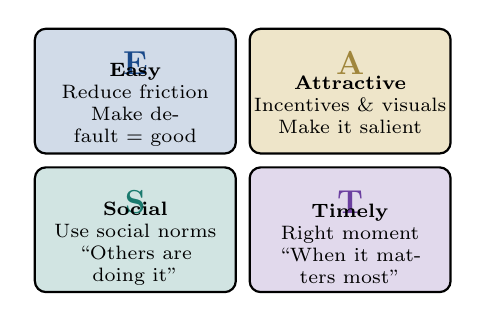
\begin{tikzpicture}[scale=0.88]
\draw[fill=beblue!20,rounded corners,thick] (-3,1.2) rectangle (-0.1,3);
\draw[fill=begold!30,rounded corners,thick] (0.1,1.2) rectangle (3,3);
\draw[fill=beteal!20,rounded corners,thick] (-3,-0.8) rectangle (-0.1,1.0);
\draw[fill=bepurple!20,rounded corners,thick] (0.1,-0.8) rectangle (3,1.0);
\node[font=\bfseries,beblue] at (-1.55,2.5) {\large E};
\node[font=\scriptsize,text width=2.5cm,align=center] at (-1.55,1.9) {\textbf{Easy}\\ Reduce friction\\ Make default = good};
\node[font=\bfseries,begold!80!black] at (1.55,2.5) {\large A};
\node[font=\scriptsize,text width=2.5cm,align=center] at (1.55,1.9) {\textbf{Attractive}\\ Incentives \& visuals\\ Make it salient};
\node[font=\bfseries,beteal] at (-1.55,0.5) {\large S};
\node[font=\scriptsize,text width=2.5cm,align=center] at (-1.55,-0.1) {\textbf{Social}\\ Use social norms\\ ``Others are doing it''};
\node[font=\bfseries,bepurple] at (1.55,0.5) {\large T};
\node[font=\scriptsize,text width=2.5cm,align=center] at (1.55,-0.1) {\textbf{Timely}\\ Right moment\\ ``When it matters most''};
\end{tikzpicture}
\column{0.47\textwidth}
\begin{block}{BIT (Behavioural Insights Team)}
Founded in UK Cabinet Office, 2010. Now in 31 countries. Runs 750+ RCTs per year across government services. ``The Nudge Unit.''
\end{block}
\begin{exampleblock}{EAST in Action}
\begin{itemize}
  \item \textbf{Easy:} Pre-fill OSAP with CRA data.
  \item \textbf{Attractive:} Colourful energy efficiency labels.
  \item \textbf{Social:} ``Your neighbours recycled 80\% this month.''
  \item \textbf{Timely:} Text vaccine reminder 3 days before your appointment.
\end{itemize}
\end{exampleblock}
\end{columns}
\end{frame}

% ============================================================
\begin{frame}{Canadian Government Nudge Policy}
\textcolor{beblue}{\textbf{Impact Canada --- Behavioural Insights Team (2018--):}}
\begin{itemize}\small
  \item \textbf{Veterans:} Simplified application $\Rightarrow$ $+$40\% uptake.
  \item \textbf{Employment Insurance:} Clear letters $\Rightarrow$ $+$20\% faster resolution.
  \item \textbf{Cancer Society:} Text reminders $\Rightarrow$ $+$30\% screening bookings.
  \item \textbf{CRA tax:} Social norm message $\Rightarrow$ $-$10\% late filing.
  \item \textbf{Canada Learning Bond:} One-click RESP $\Rightarrow$ 15\% $\to$ \textbf{52\%} takeup.
\end{itemize}
\begin{alertblock}{Principles}
\begin{enumerate}\small
  \item All interventions require RCT evidence.
  \item Transparent; evaluated for persistence; pre-registered.
\end{enumerate}
\end{alertblock}
\end{frame}

% ============================================================
\begin{frame}{[GAME] Norm Messaging Competition}
\begin{alertblock}{Group Exercise --- Write the Best Norm Message}
Each group writes a \textbf{one-sentence norm message} to encourage UNBC students:
\begin{itemize}
  \item \textbf{Group A:} Return library books on time.
  \item \textbf{Group B:} Use reusable cups at Tim Hortons.
  \item \textbf{Group C:} Get vaccinated before fall semester.
  \item \textbf{Group D:} Attend professor office hours.
\end{itemize}
\end{alertblock}
\begin{block}{Evaluation}
Class votes on most effective message. After voting, discuss:
\begin{itemize}
  \item Does it use a descriptive norm (``most students...'') or injunctive (``students should...'')?
  \item Is there a risk of boomerang? How would you prevent it?
  \item Is it timely and salient?
  \item What evidence type (RCT, field experiment, survey) would you use to test it?
\end{itemize}
\end{block}
\end{frame}

% ============================================================
\begin{frame}{Applications --- Health and Environment}
\begin{columns}
\column{0.5\textwidth}
\begin{block}{Health}
\begin{itemize}
  \item \textbf{Cafeteria design:} fruit at eye level $\Rightarrow$ 35\% more consumed.
  \item \textbf{Plate size:} smaller plates $\Rightarrow$ 30\% less food served.
  \item \textbf{Vaccine reminders + implementation intention:} ``Your appointment: Monday 2pm, Clinic X'' $\Rightarrow$ 15\% uptake increase (Milkman et al., 2021).
  \item \textbf{Stair prompts:} footprints on stairs $\Rightarrow$ +25\% stair use.
\end{itemize}
\end{block}
\column{0.47\textwidth}
\begin{block}{Environment}
\begin{itemize}
  \item \textbf{Green energy default} (UK, Germany): 7\% opt-in vs 69\% opt-out --- same energy, different default.
  \item \textbf{Vancouver plastic bag charge} (2021): 80\% reduction in single-use bags.
  \item \textbf{Carbon footprint on receipts} (Doconomy/Mastercard): CO$_2$ per purchase visible at checkout.
  \item \textbf{Real-time dashboards:} Nest/Ecobee smart thermostats show live energy cost.
\end{itemize}
\end{block}
\end{columns}
\end{frame}

% ============================================================
\begin{frame}{Applications --- Finance}
\begin{block}{Financial Nudges: What the Evidence Shows}
\begin{itemize}
  \item \textbf{TFSA default to balanced ETF} (not cash): TD pilot 2020 $\Rightarrow$ \textbf{35\% more invested}. Inertia works in your favour once the default is changed.
  \item \textbf{Credit card minimum payment warning} (FCAC 2021): Disclosing ``you will pay off this balance in X years'' $\Rightarrow$ \textbf{12\% reduction} in minimum-only payments.
  \item \textbf{Overdraft opt-in} (FCPB/credit unions 2018): Changing overdraft protection from automatic to opt-in $\Rightarrow$ \textbf{30\% reduction} in overdraft fees among frequent users.
  \item \textbf{RESP one-click enrolment} (Canada Learning Bond via CRA MyAccount): Takeup from 15\% to 52\% in pilot --- just by reducing friction.
\end{itemize}
\end{block}
\begin{exampleblock}{The Common Thread}
Every successful financial nudge either \textbf{changes the default}, \textbf{reduces friction}, or \textbf{makes long-run costs salient}. None restricts choice.
\end{exampleblock}
\end{frame}

% ============================================================
\begin{frame}{Discussion Questions}
\begin{enumerate}
  \item[\textcolor{bepurple}{Q1.}] ``Is it manipulative for governments to use defaults to increase organ donation? What if \textit{you} didn't want to donate and forgot to opt out?''
  \medskip
  \item[\textcolor{beteal}{Q2.}] ``Should corporations be \textit{banned} from using nudges against consumers? Or is this just marketing --- and where is the line?''
  \medskip
  \item[\textcolor{berust}{Q3.}] ``Design one nudge for UNBC that could improve either student health, academic outcomes, or sustainability. What evidence would you need before scaling it?''
\end{enumerate}
\end{frame}

% ============================================================
\begin{frame}{Key Takeaways --- Lecture 9}
\begin{itemize}
  \item[\textcolor{beteal}{\checkmark}] \textbf{Choice architecture is unavoidable} --- the question is only whether it is designed thoughtfully.
  \item[\textcolor{beteal}{\checkmark}] \textbf{Nudges:} libertarian paternalism --- preserve freedom while steering toward better outcomes.
  \item[\textcolor{beteal}{\checkmark}] \textbf{Defaults:} most powerful nudge. Organ donation (99.9\% vs 12\%), pension (86\% vs 49\%).
  \item[\textcolor{beteal}{\checkmark}] \textbf{Framing:} same information, different presentation $\Rightarrow$ different choices.
  \item[\textcolor{beteal}{\checkmark}] \textbf{Social norms:} descriptive + injunctive norms shift behaviour; beware boomerang.
  \item[\textcolor{beteal}{\checkmark}] \textbf{EAST Framework:} Easy, Attractive, Social, Timely.
  \item[\textcolor{beteal}{\checkmark}] \textbf{Canadian nudge policy:} Impact Canada, CRA, FCAC --- real, evidence-based, measurable.
\end{itemize}
\medskip\textcolor{beblue}{\textbf{Next:}} \textbf{Lecture 10: Applications \& Policy Design} --- Bringing it all together. When should we use nudges vs taxes vs mandates? How do we evaluate behavioural policies? And what are their limits?
\end{frame}

\end{document}
